 (DLT) method, the Levenberg-Marquardt algorithm, and the RANSAC algorithm. \n\n\\begin{figure}[htb]\n    \\centering\n    \\includegraphics[width=0.5\\textwidth]{example-image-a}\n    \\caption{Perspective-N-Point(PnP) Problem}\\label{F:test-a}\n\\end{figure}\n\n\n\\subsection{Kalman Filter}\nUsing face position provided by pnp solver directly usually is an effeient way, but not stable enough to cover noises from possible environments.  Since keypoints provided by detector is not stable enough to get a steady result, position solve by pnp-solver often meet unexpected oscillation and jittering. To solve the problem, we introduce kalman filter as a filter to smooth the movement of human head. \n\nKalman Filter is a specific type of recursive Bayesian filter, which is used to estimate the state of a linear dynamic system from a series of noisy measurements. As a varietas of Bayesian filter, Kalman filter combain the prior knowledge of the system with the current measurement to provide an optimal estimate of the state of the system by a self-adjusting kalman gain $K$. \n\nThe Kalman Filter is based on a linear dynamical system model, based on following elements:\n\\begin{itemize}\n    \\item State Vector $x_k$: State to be estimated of the  system.\n    \\item Measurement Vector $z_k$: Variable can be measured by sensors of the system. Note the measurement is noisy.\n    \\item State Transition Matrix $F_k$: State transition matrix, which describe the state transition of the system from prior state to current state.\n    \\item Measurement Matrix $H_k$: Measurement matrix, which describe the mapping from state space to measurement space.\n    \\item Process Noise Covariance Matrix $Q_k$: Covariance matrix of the process noise.\n    \\item Measurement Noise Covariance Matrix $R_k$: Covariance matrix of the measurement noise.\n    \\item Kalman Gain $K_k$: Gain of the Kalman filter, which is used to adjust the weight of the prior state and the measurement.\n    \\item State Covariance Matrix $P_k$: Covariance matrix of the prior state.\n\\end{itemize}\n\nThe Kalman Filter consists of two main steps: the prediction step and the update step. In the prediction step, filter predict the state of the system based on the prior state and the state transition matrix and update prior state covariance P:\n\\begin{equation}\n    \\hat{x}_{k|k-1} = F_k \\hat{x}_{k-1|k-1} \n\\end{equation}\n\\begin{equation}\n    P_{k|k-1} = F_k P_{k-1|k-1} F_k^T + Q_k\n\\end{equation}\n\n\nOnce the measurement is available, the filter update the state of the system based on the measurement and the measurement matrix:\n\\begin{equation}\n        K_k = P_{k|k-1} H_k^T (H_k P_{k|k-1} H_k^T + R_k)^{-1}\n\\end{equation}\n\\begin{equation}\n        \\hat{x}_{k|k} = \\hat{x}_{k|k-1} + K_k(z_k - H_k \\hat{x}_{k|k-1})\n\\end{equation}\n\\begin{equation}\n        P_{k|k} = (I - K_k H_k) P_{k|k-1} \n\\end{equation}\n\nIn update step, kalman gain is updated based on the measurement and the prior state covariance, and providing the optimal estimate of the state of the system in next step.\n\n\\subsection{Perspective Projection and Off-axis Perspective Projection}\n\nPerspective projection is a common projection method in computer graphics and daily life. It is used to project a 3D point onto a 2D plane. Consider a 3d object point, perspective projection generated 2d coordinate by mapping it to a 2 * 2 * 2 rectangular-projection cube, where $x$ and $y$ are the 2D position and $z$ is the depth information of the 3D point(Figure 10a).\n\nAs camera field of view($fov$) given, we can generate the perspective projection matrix as:\n\n\\[\n\\begin{bmatrix}\n\\frac{\\cot \\left( \\frac{\\text{fovy}}{2} \\right)} {aspect} & 0 & 0 & 0 \\\\\n0 & \\cot \\left( \\frac{\\text{fovy}}{2} \\right) & 0 & 0 \\\\\n0 & 0 & -\\frac{f+n}{f-n} & -\\frac{2fn}{f-n} \\\\\n0 & 0 & -1 & 0\n\\end{bmatrix}\n\\]\nWhere $f$ is the far plane, $n$ is the near plane, and $aspect$ is the aspect ratio of the view plane. Fully explanation of perspective projection can be found in \\cite{ahn_opengl_projection_matrix}.\n    \n\n\\begin{figure}[htb]\n    \\centering\n\n    \\begin{subfigure}[t]{.45\\linewidth}\n        \\centering\n        \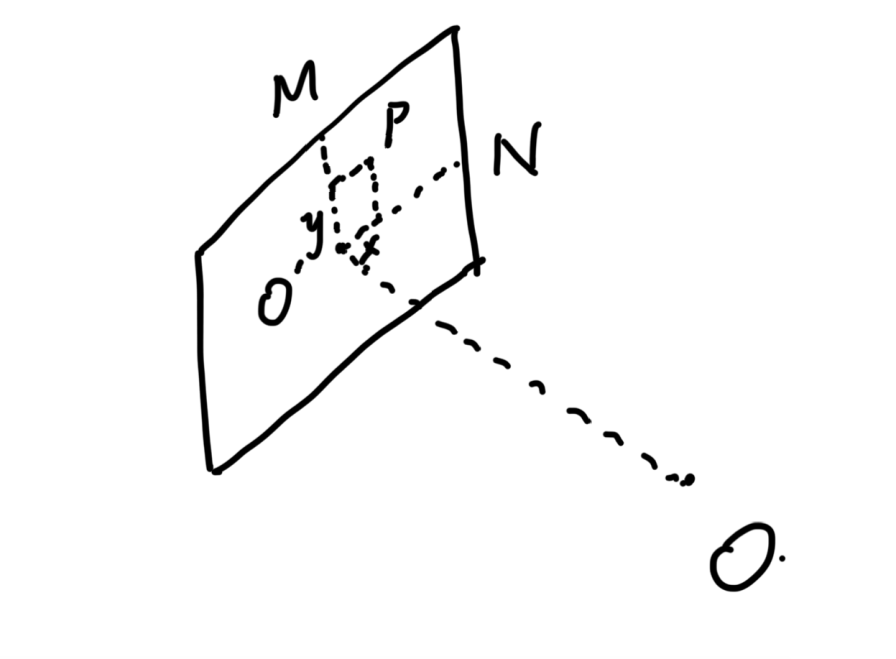
\includegraphics[width=1\\textwidth]{figures/Preliminaries/perspective.png}\n        \\caption{Pinhole camera model, where $O$ is ovserver's position, $O'$ is view point, $O'MN $ is view plane, $P$ is the 2D projection on view plane of a 3D point, and $M$, $N$ is the orthogonal projection from the viewpoint to the upper/right boundary of the plane.}\\label{F:test-a}\n    \\end{subfigure}\n\n    \\begin{subfigure}[t]{.45\\linewidth}\n        \\centering\n        \\includegraphics[width=1\\textwidth]{example-image-a}\n        \\caption{The target of perspective project is mapping 3D points to a 2 * 2 * 2 cube, where x and y are the related 2D coordinate and z is the depth information of the 3D point.}\\label{F:test-b-sub-a}    \\end{subfigure}\n    \\caption{}\\label{F:test-b}\n\\end{figure}\n\nHowever, perepective projection assumes that the camera is always facing the view plane directly(OO' prpendicular to plane MO'N), which is not always the case in real life. In some cases, the camera may be facing the view plane at an angle(Figure 1). To provide a more realistic view of the scene, off-axis perspective projection is proposed\\cite{off-axis}\\cite{Kooima2011GeneralizedPP}. By assuming the camera is facing the view plane at an angle, off-axis perspective projection calculate axis's angle by the intersection point's 2D coordinate in view plane(Figure), and provide a rotate-include projection matrix to project 3D point to 2D plane. \n\n\nOff-axis projection calculate projection matrix by additional distances from view point to view plane's boundary($r, r, t, b$ in Figure 11b). The projection matrix can be calculated as:\n\n\\[\n\\begin{bmatrix}\n\\frac{2n}{r-l} & 0 & \\frac{r+l}{r-l} & 0 \\\\\n0 & \\frac{2n}{t-b} & \\frac{t+b}{t-b} & 0 \\\\\n0 & 0 & -\\frac{f+n}{f-n} & -\\frac{2fn}{f-n} \\\\\n0 & 0 & -1 & 0\n\\end{bmatrix}\n\\]\n\nSimilarly, derivation details can be found in \\cite{Kooima2011GeneralizedPP}.\n\nFigure 11b shows why off-axis projection is needed. About the situation of our research, actual view plane is user's display monitor, which is not perpendicular to the user's line of sight most of the time.\n\n\n\\begin{figure}[htb]\n    \\centering\n    \\begin{subfigure}[t]{.45\\linewidth}\n        \\centering\n        \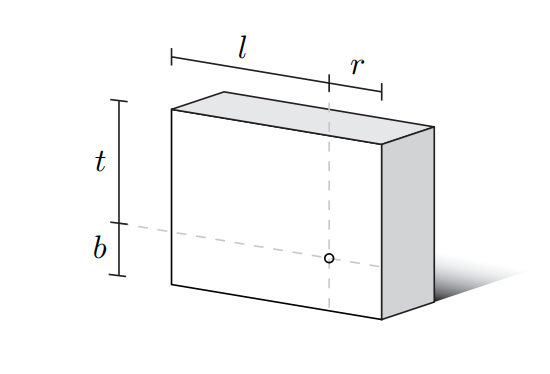
\includegraphics[width=1\\textwidth]{figures/Preliminaries/off-axis.png}\n        \\caption{Off-axis projection}\\label{F:test-b-sub-a}\n    \\end{subfigure}\n    \\begin{subfigure}[t]{.45\\linewidth}\n        \\centering\n        \\includegraphics[width=1\\textwidth]{example-image-a}\n        \\caption{Why off-axis projection is needed}\\label{F:test-b-sub-b}\n    \\end{subfigure}\n    \\caption{}\\label{F:test-b}\n\\end{figure}",
 "\\part{Method and Experiment}\n\n\\section{Method}\n\nTo implemented the proposed system, we divide the system into three main parts: head tracking, 3D effect, and curved display corrention. In Section4.1, we introduce the basic structure of algorithm and the intra-process communication framework used. Section4.2 introduced head tracking part, which is responsible for tracking the user's head movement and providing the user head's position and do filter. Section4.4 introduce methods and details about how to implement 3D effect, including unity simulation part and off-axis projection implementation. Section4.4 introduce the curved display correction, which is responsible for correcting the image distortion on the curved display.\n\n\\subsection{Framework}\nSystem's framework can be devided into two parts in platform level: C++ level and Unity level. C++ level is responsible for head tracking and image correction, and Unity level is responsible for off-axis projection and simulation constructing. The communication between C++ and Unity is based on Robot Operating System 2(ROS2)\\cite{ros2} and Unity's ROS2 plugin\\cite{ros2forunity}, since ros2 provided a convinience way to both communication and data visualization. Code structure is shown in Figure 12.\n\n\\begin{figure}[htb]\n    \\centering\n    \\includegraphics[width=0.5\\textwidth]{example-image-a}\n    \\caption{code structure and working-flow}\\label{F:test-a}\n\\end{figure}\n\nIn detector, we use YuNet\\cite{Wu_2023} to detect the user's face and get the face's key points. Then keypoints is sent to pnp solver, which return head's position in camera frame and send to tracker. Tracker node process head's position, applying CV motion model to kalman filter and send result to Unity part. In Unity, we have constructed a simulation environment, which include two position-synchronized cameras to simulate the movement combination of rendering camera and human head. Render result will be sent to wrap node, which apply finally image correction and send to display.\n\nTo achieve a sufficiently immersive effect, it is essential to:\n\\begin{itemize}\n    \\item Ensure a stable head position to prevent the resultant image from shaking.\n    \\item Minimize system processing time to enable fast response in real-time 3D systems.\n    \\item Provide reliable image correction to prevent distortion on curved displays.\n\\end{itemize}\n\n\\subsection{Head Tracking}\nIn head tracking part, we use YuNet\\cite{Wu_2023} to detect the user's face and get the face's key points, and applying CV motion model to do filter.\n\n\\subsubsection{Detector and Locator}\nOpenCV 4.5.4\\cite{opencv_4_5_4} have integrated YuNet as one of face landmark detection function. Network structure of YuNet is shown in Figure 13. \\footnote[1]{Onnx model file can be found at \\href{https://github.com/opencv/opencv_zoo/tree/main/models/face_detection_yunet}{OpenCV Model Zoo}}\n\n\\begin{figure}[htb]\n    \\centering\n    \\includegraphics[width=0.5\\textwidth]{example-image-a}\n    \\caption{YuNet network structure}\\label{F:test-a}\n\\end{figure}\n\nIn OpenCV's API, YuNet accept a RGB image as input, and return a n * 14 size matrix, while n is the number of faces detected in the image. For each row, the first 4 elements are the bounding box of the face, and the rest 10 elements are the key points of the face, representing right eye, left eye, nose, right chin and left chin.\n\n For localization, OpenCV also privide solvePnP() as a pnp solve api. Since solvePnP() function return camera's pose in world frame, we defined face-frame pnp's world frame(Figure 14).\n\n\n\nFor localization, OpenCV also provide solvePnP() as a pnp\n solve api, with input of 3d points(world frame), 2d points(opencv's image frame), camera matrix and distortion matrix as input, output of camera's pose in world frame. Since solvePnP() function return camera's pose in world frame, world frame is defineded same as face-frame. Figure 14 shows the face-frame definition.\n\n\\begin{figure}[htb]\n    \\centering\n    \\includegraphics[width=0.5\\textwidth]{example-image-a}\n    \\caption{Face-frame definition}\\label{F:test-a}\n\\end{figure}\n\nIn addition, ePnP is chosen by its low-latency\\cite{EPnP_2009}. Also, we've obtained camera's intrinsic matrix and distortion matrix by ros2 camera calibration package\\cite{ros2_camera_calibration}, and applicated 3d-keypoints in a sample human head's model from Soheil M. etc(2023)'s work.\\cite{soheil2023facial}\n\n\\subsubsection{Kalman Filter Design}\nConsider the general movement of human head, we choose Kalman Filter as our motion model, since the head movement is a linear dynamic system. The state variables can be defined as head's:\n$$\nx_k = \\begin{bmatrix} x & y & z & v_x & v_y & v_z \\end{bmatrix}^T\n$$\n\n$$\nz_k = \\begin{bmatrix} x & y & z \\end{bmatrix}^T\n$$\n\nwhile $x, y, z$ is the position of the head, and $v_x, v_y, v_z$ is the velocity of the head. \nConsider head's movement as a constant velocity(cv) model, the state transition equations can be defined as:\n$$\n\\begin{cases}\n    x' = x + v_{x} \\cdot dt \\\\\n    y' = y + v_{y} \\cdot dt \\\\\n    z' = z + v_{z} \\cdot dt \n\\end{cases}\n$$\nand observation equations:\n$$\n\\begin{cases}\n    x_m = x \\\\\n    y_m = y \\\\\n    z_m = z\n\\end{cases}\n$$\n\nwhile $x_m, y_m, z_m$ are variables in measurement space, and $dt$ is the time interval between two frames. \n\nIn this case, we can generate the state transition matrix $F_k$ and measurement matrix $H_k$ as:\n\n$$    \nF_k = \\begin{bmatrix} 1 & 0 & 0 & dt & 0 & 0 \\\\ 0 & 1 & 0 & 0 & dt & 0 \\\\ 0 & 0 & 1 & 0 & 0 & dt \\\\ 0 & 0 & 0 & 1 & 0 & 0 \\\\ 0 & 0 & 0 & 0 & 1 & 0 \\\\ 0 & 0 & 0 & 0 & 0 & 1 \\end{bmatrix} \n$$\n$$\nH_k = \\begin{bmatrix} 1 & 0 & 0 & 0 & 0 & 0 \\\\ 0 & 1 & 0 & 0 & 0 & 0 \\\\ 0 & 0 & 1 & 0 & 0 & 0 \\end{bmatrix}\n$$\n\nBy given the process noise covariance matrix $Q_k$ and measurement noise covariance matrix $R_k$ a proper value, we can apply Kalman Filter to track the head's position.\n\n\\subsubsection{Target Lost and Target Switch}\nIn most cases, tracking algorithm can works well and provide a reliable result. However, target lost will happen in minority of situation, since face landmark detector may fail or traking target switches, which may lead to an abnormal condition since filter will update its sta by a wrong measurement. To handle this condition, an additional threshold variable is set to determine whether the measurement position is reliable. For each frame, the predict step and update step of kalman filter is divided, and the update step will only be executed when the measurement is close enough to the prediction, otherwise reset $x,y,z$ to prediction and $v_x,v_y,v_z$ to 0.\n\n\n\\subsection{Simulation}\n\nThe simulation part is developed in Unity, a responsible graphic engine which is widely used in film and game industry. Simulation environment is devided into two sub-parts: user part and render part.\n\\begin{itemize}\n    \\item \\textbf{User Part}: contains one viewing camera object and one plane object. Viewing camera's transform is synchronized with user head's position by subscribe to tracker node with the support of ROS2ForUnity. Plane object is by a specific meterial, to display render result from render camera.\n    \\item \\textbf{Render Part}: contains one render camera and some example objects. Render camera is processed by an off-axis projection matrix, and will motion is synchronized with viewing camera. Render camera will also publish result image by ros2 component for correction algorithm. Example objects are used to test the 3D effect.\n\\end{itemize}\n\n\\begin{figure}[htb]\n    \\centering\n    \\includegraphics[width=0.5\\textwidth]{example-image-a}\n    \\caption{Simulation Environment Structure}\\label{F:test-a}\n\\end{figure}\n\nA generate working flow is shown in Figure 15. Each steps are described as follows:\n\\begin{itemize}\n    \\item \\textbf{Step 1}: Viewing camera receive head's position from tracker node, and update position.\n    \\item \\textbf{Step 2}: Render camera take a motion, to adjust its position to simulate the user's head movement.\n    \\item \\textbf{Step 3}: Camera rendering the scene with off-axis projection matrix, and publish it by publisher provided by its ros2 component.\n    \\item \\textbf{Step 4}: Material in screen plane update, viewing camera publish the image as a ros topic to show the illusion when screen have no distortion.\n\\end{itemize}\n\nCoordinate of these two part are also synchronized by two anchor points. Anchors performs as two parts coordinates' origin. By this way, objects in two parts can use same relative coordinates, and get a better performance when position synchronize.\n\n\\subsection{Curved Displays Correction}\nAccording to the user's different three-dimensional coordinates in space, the visual effect of the screen shape changes accordingly. This technique only considers the horizontal deformation of the screen, referred to here as the visual angle. Define the center of the curved screen as the origin \\( O(0,0) \\), with point \\( A \\) on the left and point \\( B \\) on the right of the screen, the radius of curvature as \\( r \\), and the central angle of the curved screen as \\( \\beta \\). The user's eye position in the two-dimensional coordinate system is \\( N(a,b) \\), and the number of equal divisions of the screen \\( n \\) (within a certain range, the larger the parameter \\( n \\), the better the visual effect). The user's current visual angle \\( \\alpha \\) can be calculated as follows:\n\n\\begin{figure}[htb]\n    \\centering\n    \\includegraphics[width=0.8\\textwidth]{figures/Implementation/corection.png}\n    \\caption{Curved Display Correction}\\label{F:test-a}\n\\end{figure}\n\nFrom the three-dimensional coordinates of the user's eye position \\( U(x_u, y_u, z_u) \\), the three-dimensional coordinates of the screen center \\( V(0, 0, \\frac{h_s}{2}) \\) (where \\( h_s \\) is the actual screen height) are obtained. Considering only the horizontal visual angle and ignoring the z-coordinate, define the center of the curved screen as the origin \\( O(0,0) \\), with point \\( A \\) on the left and point \\( B \\) on the right of the screen. Suppose the radius of curvature is \\( r \\), the central angle of the curved screen is \\( \\beta \\), and the user's eye position in the two-dimensional coordinate system is \\( N(a, b) \\) (where \\( a = x_u, b = y_u \\)). When the user looks at the screen with coordinates \\( V(x_v, y_v) \\), the current visual angle \\( \\alpha \\) can be calculated as follows:\n\n\\begin{equation}\n\\alpha = \\arccos \\left( \\frac{\\overline{NA} \\cdot \\overline{NB}}{|\\overline{NA}||\\overline{NB}|} \\right)\n\\end{equation}\n\nThe vectors \\( \\overline{NA} \\) and \\( \\overline{NB} \\) can be expressed as follows:\n\n\\begin{equation}\n\\overline{NA} = (p, q) = \\left( -r \\sin \\frac{\\beta}{2} - a, r \\cos \\frac{\\beta}{2} - r - b \\right) \n\\end{equation}\n\n\\begin{equation}\n\\overline{NB} = (o, q) = \\left( r \\sin \\frac{\\beta}{2} - a, r \\cos \\frac{\\beta}{2} - r - b \\right)\n\\end{equation}\n\nDividing the visual angle \\( \\alpha \\) into \\( n \\) equal parts, define the intersections of the equal division lines with the screen as \\( a_1, a_2, \\ldots, a_n \\) (where point \\( A \\) is \\( a_0 \\), point \\( B \\) is \\( a_n \\)). The coordinates of \\( a_i \\) are noted as \\( (x_i, y_i) \\):\n\n\\begin{align}\n    y_i - b &= k_i(x_i - a)\n\\end{align}\n\\begin{align}\n    x_i^2 + (y_i + r)^2 &= r^2 \n\\end{align}\n\nFrom equations (9) and (10), we get:\n\n\\begin{align}\ny_i = \\frac{|k_i| \\sqrt{-a^2k_i^2 + 2abk_i + 2ak_ir - b^2 - 2br + k_i^2r^2} - ak_i + b - k_i^2r}{k_i^2 + 1} \n\\end{align}\n\\begin{align}\n    x_i = a + \\frac{y_i - b}{k_i}\n\\end{align}\n\nwhere \\( k_i \\) is the slope of line \\( N a_i \\), calculated as follows:\n\n\\begin{equation}\nk_i = \\tan \\left( -\\frac{i \\alpha}{n} + \\arctan \\left( \\frac{q}{p} \\right) \\right) \n\\end{equation}\n\nOnce all coordinates \\( a_1, a_2, \\ldots, a_n \\) are obtained, we can calculate the length of each divided segment:\n\n\\begin{equation}\na_i a_{i+1} = \\left( \\arctan \\left( \\frac{y_i + r}{x_i} \\right) - \\arctan \\left( \\frac{y_{i+1} + r}{x_{i+1}} \\right) \\right) r \n\\end{equation}\n\nThus, the ratio of the deformed segments to the corresponding screen segments can be defined as \\( r_n \\):\n\n\\begin{equation}\nr_n = \\frac{n a_i a_{i+1}}{\\overline{AB}}\n\\end{equation}\n\nwhere\n\n\\begin{equation}\n\\overline{AB} = \\beta r\n\\end{equation}\n\nAccording to the obtained results, the corresponding parts of the deformed screen can be proportionally stretched or shrunk to achieve the desired screen deformation effect.\n\n\n\\section {Experiment}\n\n\\subsection{Measurement of Head Tracking}\n\n\\subsection{Algorithm speed}\n\\subsection{Illusion Effects}\n\n\n\\subsection{Curved Displays Correction}\n\n\n"]